\documentclass[preprint, authoryear, 10 pt]{sigplanconf}

\setpagenumber{1}

\usepackage{comment}

%% \usepackage[style=alphabetic]{biblatex}
%% \usepackage[authoryear]{natbib}
%% \PassOptionsToPackage{authoryear}{natbib}
%% \usepackage{caption}
\usepackage{graphicx}
\usepackage{subfigure}
\usepackage{url}

\usepackage{paralist}
\usepackage[pdfpagelabels]{hyperref}
\usepackage[all]{hypcap}
\usepackage{verbatim}
\usepackage{array}
\usepackage{float}
\usepackage{multirow}
% \usepackage{rotating}
\usepackage{multicol}
\usepackage{longtable}

\usepackage{listings} 	
% "define" Scala
\lstdefinelanguage{scala}{
  morekeywords={abstract,case,catch,class,def,%
    do,else,extends,false,final,finally,%
    for,if,implicit,import,match,mixin,%
    new,null,object,override,package,%
    private,protected,requires,return,sealed,%
    super,this,throw,trait,true,try,%
    type,val,var,while,with,yield},
  otherkeywords={=>,<-,<\%,<:,>:,\#,@, <:<},
  sensitive=true,
  morecomment=[l]{//},
  morecomment=[n]{/*}{*/},
  morestring=[b]",
  morestring=[b]',
  morestring=[b]"""
}

\usepackage{pxfonts}
\usepackage{color}
\definecolor{dkgreen}{rgb}{0,0.6,0}
\definecolor{gray}{rgb}{0.5,0.5,0.5}
\definecolor{mauve}{rgb}{0.58,0,0.82}
 
% Default settings for code listings
\lstset{frame=tb,
  language=scala,
  aboveskip=3mm,
  belowskip=3mm,
  showstringspaces=false,
  columns=flexible,
  basicstyle={\small\ttfamily},
  numbers=left, % none,
  numbersep=2pt,
  numberstyle=\tiny\color{gray},
  keywordstyle=\bfseries\color{blue},
  commentstyle=\color{dkgreen},
  stringstyle=\color{mauve},
  frame=none, % single,
  breaklines=true,
  breakatwhitespace=true,
  tabsize=2,
  captionpos=b
}

% A comment in a draft (shouldn't appear in the final version).
\newcommand{\mycomment}[1]{\(\spadesuit\){\bf #1 }\(\spadesuit\)}
% Comment this out in the draft
% \newcommand{\mycomment}[1]{}
\newcommand{\pmcomment}[1]{\comment{PM}{#1}}
\newcommand{\pwtcomment}[1]{\comment{PT}{#1}}
\newcommand{\rscomment}[1]{\comment{RS}{#1}}

% line break in table.  e.g.
% Foo bar & \specialcell{Foo\\bar} & Foo bar \\    % vertically centered
% Foo bar & \specialcell[t]{Foo\\bar} & Foo bar \\ % aligned with top rule
\newcommand{\specialcell}[2][c]{%
  \begin{tabular}[#1]{@{}c@{}}#2\end{tabular}}

\permission {[Copyright notice will appear here once ’preprint’ option is removed.]}

\begin{document}

\frontmatter          % for the preliminaries

\title{Type-parameterized Actors and Their Supervision (v6.6.5) } % title

\authorinfo{Jiansen HE}
           {University of Edinburgh}
           {jiansen.he@ed.ac.uk}
\authorinfo{Philip Wadler}
           {University of Edinburgh}
           {wadler@inf.ed.ac.uk}
\authorinfo{Philip Trinder}
           {University of Glasgow}
           {P.W.Trinder@glasgow.ac.uk}

% \category{I.3.7}{Computer Graphics}{Three-Dimensional Graphics and Realism}[Animation]
% \category{I.3.5}{Computer Graphics}{Computational Geometry and Object Modeling}[Physically based modeling]

% \terms{Experimentation, Human Factors}



\maketitle



\begin{abstract} 
The robustness of distributed message passing applications can be improved by
\begin{inparaenum}[(i)]
 \item employing failure recovery mechanisms such as the supervision principle, or
 \item using typed messages to prevent ill-typed communication.
\end{inparaenum}
The former approach is originally developed in the Erlang OTP (Open Telecom 
Platform) library.  The later approach has been well explored in systems 
including the join-calculus and the typed $\pi$-calculus.  Attempts of combing 
those two approaches has been made in two directions: type checking existing 
Erlang programs and implementing a statically typed actor library that supports 
the supervision principle.   Unfortunately, current statically typed actor 
libraries either use dynamically typed messages (e.g. Akka), or do not support 
supervision (e.g. Cloud Haskell).

Implementing a statically typed actor library that also supports the 
supervision principle raises three problems. Firstly, distributed resources are 
dynamically typed whereas local implementation is statically type checked and 
does not need to consider ill-typed messages.  Therefore, a mixture of statical 
and dynamical type checking is required to make sure that distributed resources 
are well-typed.  Secondly, preventing unexpected messages to an actor requires 
that actor having different types when it communicates with others.  Thirdly, 
an elegant notion of sub-typing is required for the supervision purpose so that 
a supervisor can interact with child actors of different types, even in systems 
where sub-typing is not directly supported.




\begin{comment}
Implementing a statically typed actor library that also supports the 
supervision principle raises three problems.  Firstly, current design of name 
servers are dynamically typed and do not map typed names to resources of 
corresponding types.  Therefore, a novel typed name server is required.  
Secondly, actors cannot be naively parameterized by the union type of all 
expected message types, including those for supervision purposes, because 
supervisors must interact with child actors of different types.  Thirdly, 
unexpected messages can be sent to actors which publish more type information 
than necessary to other parties.
\end{comment}

This paper introduces the typed Akka library, TAkka, which resolves above
problems. Although TAkka actor extends Akka actor and use the Scala 
{\tt Manifest} class to serialize type information, we believe that similar 
improvements 
can be made to actor libraries in other languages.

We evaluate the TAkka library by re-implementing examples built from small and 
medium sized Erlang and Akka libraries.  Results show that Akka programs can be gradually upgraded 
to TAkka equivalents with minimal runtime and code size overheads.  
TAkka programs have similar scalability to their Akka equivalents. 
Finally, we port the Chaos Monkey library for assessing application reliability 
and design a Supervision View library for dynamically capturing the structure 
of supervision trees.

\begin{comment}
This paper presents the design, implementation and preliminary evaluation
results of the TAkka library, where types of actor related components are
statically typed and operations are type checked at the earliest possibility.
We introduce actors parameterized by the type of messages they expect to
receive. We show that it is straightforward to construct
supervision trees of type-parameterized actors. We minimize the number of system
messages that may be handled by general users by providing standard supervision
strategies.


\end{comment}


\end{abstract}

\category{D.1.3}{Programming Techniques}{Concurrent Programming}

\terms
Design, Languages, Reliability

\keywords
actor, type, supervision tree, name server


\section{Project Description}

\subsection{Background and Motivation}

Concurrent programming is facing new challenges due to the recent advent of multi-core processors, which rely on parallelism, and the pervasive demands of web applications, which rely on distribution.  Theoretic works on concurrency can be traced back to Petri net and other approaches invented in 1960s \cite{historyPA}.  Since 1980, more attention has been paid to the study of process calculi (a.k.a. process algebras), which provide a family of formal models for describing and reasoning about concurrent systems \cite{abramsky}.  The proliferation of Process Calculi marks the advance in concurrency theory.  ``The Dreams of Final Theories'' \cite{abramsky} for concurrency, however, have not been achieved.

In practice, it is difficult to build a reliable distributed system because of its complexity.  Firstly, a distributed system shares features and problems with other concurrent systems.  For instance, it is non-deterministic so that traditional input-output semantics is inadequate to be used for reasoning about its behaviour.  Secondly, scalability of a distributed system is usually a challenge for its developers.  For example, developers of a distributed system are unlikely to know the structure of the system in advance.  Moreover, the mobility \cite{MobileAmbients} of a distributed system requires the capability of changing its topological structure on the fly.  In addition, the latency of communication could be affected by many unpredictable factors.  Thirdly, the system should be tolerant of partial failures.  For example, when a site fails to respond to messages,  the system should address this failure by invoking a recovery mechanism.   	

Fortunately, some recent works provide a solid basis for the design of distributed programming languages.  For example, the ambient calculus \cite{MobileAmbients} models the movement of processes and devices.  Bigraphs \cite{bigraph_book}, a more abstract model, is aiming at describing spatial aspects and mobility of ubiquitous computing.  Session types \cite{Honda93typesfor, Honda_languageprimitives} guarantees that two parties of a session always communicate in a dual pattern.  Lastly, the join-calculus \cite{full_join} is a remarkable calculus which models features of distributed programming as well as provides a convenient construct, the join patterns, for resources synchronisation.  It is also important to note that the syntax of the join-calculus is close to a real programming language and therefore reduces the barrier between understanding the mathematical model and employing this abstract model to guide programming practices.

In addition, good programming principles, such as the OTP design principles\footnote{OTP is stand for Open Telecom Platform.  It provides a set of libraries for developing Erlang applications.  For the above reason, it is also known as Erlang/OTP design principles}, have been developed and verified by the long-term implementation practice.  OTP is a platform for developing concurrent, distributed, fault tolerant, and non-stop Erlang applications \cite{Erlang}.  In the past 20 years, the Erlang language was used to build large reliable applications like RabbitMQ, Twitterfall, and many telecommunications systems.

Nevertheless, Erlang is an untyped functional programming language whereas a typed language detects certain forms of data misuse earlier.  Therefore, it would be pleasant to combine advantages of static typing and OTP principles.  At the time of this writing, this idea has been partly realised in the akka framework \cite{akka}.  In spite of some attempts, the akka framework inherits some limitations of using untyped actors from the Erlang programming language.  This situation left us research potentials in this line.

\subsection{Project Aim}
\label{aim}
The aim of this project is to {\it{build a library that supports OTP design principles in a typed setting}}. The project intends to explore factors that encourage programmers to employ good programming principles.  This project will demonstrate how types and appropriate models help the construction of reliable distributed systems.

\subsection{Project Objectives}
\label{objectives}

\begin{enumerate}
  \item To identify a number of medium-sized applications implemented in Erlang using OTP principles.  Those examples will be served as references to evaluate frameworks that support OTP principles.  Candidate examples shall cover a wide range of aspects in distributed programming, including but not limited to 
    \begin{inparaenum} [(a)]
      \item transmitting messages and potentially computation closures, 
      \item modular composition of distributed components, 
      \item default and extensible failure recovery mechanism, 
      \item eventually consistency model for shared states, and 
      \item dynamic topology configuration and hot code swapping.
    \end{inparaenum} 
  \item To re-implement and compare identified applications within existing frameworks.  The primitives purpose of this work is to be aware of prominent features and limitations of existing frameworks.  As a research which contains certain level of overlaps with other existing and evolving frameworks, this research should distinguish itself from others by devised solutions to some problems which are difficulty to be solved by alternatives.  Moreover, the evaluation component formalised in this work is likely to be novel for comparing frameworks aiming at supporting distributed computation.  The same evaluation component will be used for evaluating our later developed library as well.
  \item To implement a library that supports OTP design principles in a typed setting.  The library could be built either on top of existing frameworks or with lower level constructs.  It important to note that the library might be based on an abstraction that is more general than the actor model.  Although OTP design principles were proposed for the Erlang language, which is based on the Actor model, we believe that it should be possible to rephrase those good programming principles in other models.  To demonstrate the wide applications of OTP design principles, the library interface should provide a certain level of generality so that it could be implemented by and used within different models.
  \item To demonstrate how the proposed library meets the demands of distributed programming.  At this stage, the proposed library will be used to (a) demonstrate how to write small programs aiming at different requirements; (b) demonstrate its scalability of programming in the large by reimplementing applications used in objective 1 and 2.
  \item To summarise some challenges in distributed programming and how to get around those difficulties with the proposed library and other programming frameworks.  The summary will reveal how language libraries, which is used for practical purposes, are related to their theoretical guidance underneath.  It may also plot research blanks for future study.
\end{enumerate}



\section{Actor Programming}
\label{background}

\subsection{Actor Model and OTP Design Principles}

The Actor model defined by Hewitt et al.  \cite{Hewitt:1973} treats actors as
primitive computational components.  Actors collaborate by sending asynchronous
messages to each other.  An actor independently determines its reaction to
messages it receives.

The Actor model is adopted by the Erlang programming language, whose 
developers later summarized 5 OTP design principles to improve the 
reliability of Erlang applications \cite{OTP}.  We notice that the Behaviour 
principle, the Application principle, and the Release principle coincide with 
3 Java and Scala Programming practices listed in Table \ref{otp}.  The 
Release Handling principle requires runtime support for hot swapping.  In a 
platform where hot swapping is not supported in general, e.g. Java Virtual 
Machine (JVM), hot swapping a particular component can be simulated by updating 
the reference to that component. For example, Section \ref{hot_swapping} 
explains how to hot swap the behaviour of an actor in TAkka, which runs on the 
JVM. The Supervision principle, which is the central topic of this paper, 
has no direct correspondence in native JVM based systems.

\begin{table}[t]
\label{otp}
% \tbl{Implementing OTP Design Principles in an OO Language}{
 \begin{center}
\begin{tabular}{| l | p{4.5 cm} | }
\hline
  OTP Design Principle & JAVA/Scala Programming \\
\hline
  Behaviour & defining an abstract class \\
\hline
  Application  & defining an abstract class that has two abstract methods: start and stop \\
\hline
  Release  & packaging related application classes  \\ 
\hline
  Release Handling  & hot swapping support on key modules is required \\
\hline
  Supervision  & no direct correspondence  \\
\hline
\end{tabular}
 \caption[]{Using OTP Design Principles in JAVA/Scala\\  Programming}
\end{center}
%}
\end{table}




\subsection{Akka Actor}
\label{akka actor}


An Akka Actor has four essential components as shown in Figure 
\ref{fig:akka_actor_api}: (i) a receive function that defines its reaction to 
incoming messages, (ii) an actor reference pointing to  itself, (iii) the actor 
 context representing the outside world of the actor, and (iv) the supervisor 
strategy for its children.

\begin{figure}[h]
\label{fig:akka_actor_api}
\begin{lstlisting}[language=scala]
package akka.actor
trait Actor{
  def receive:Any=>Unit
  val self:ActorRef
  val context:ActorContext
  var supervisorStrategy: SupervisorStrategy
}
\end{lstlisting}
\caption{Akka Actor API}
\end{figure}

Figure \ref{akkastring} shows an example actor in Akka.  The {\tt receive} 
function of the Akka actor has type {\tt Any$\Rightarrow$Unit} but the 
defined actor, {\tt ServerActor}, is only intended to process strings.  At Line 
16, a {\tt Props}, an abstraction of actor creation, is initialized and passed 
to an actor system, which creates an actor with name \textcolor{mauve}{\tt 
server} and returns a reference pointing to that actor.  Another way to obtain 
an actor is using the {\tt actorFor} method as shown in line 24.  We then use 
actor references to send the actor string messages and integer messages.  
String messages are processed in the way defined by the receive function.

\begin{figure}[t]
 \label{akkastring}
      \begin{lstlisting}[language=scala]
class ServerActor extends Actor {
  def receive = {
    case m:String => println("received message: "+m)
  }
}

class MessageHandler(system: ActorSystem) extends Actor {
  def receive = {
    case akka.actor.UnhandledMessage(message, sender, recipient) =>
      println("unhandled message:"+message);
  }
}

object ServerTest extends App {
  val system = ActorSystem("ServerTest")
  val server = system.actorOf(Props[ServerActor], "server")
  
  val handler = system.actorOf(Props(new MessageHandler(system)))
  system.eventStream.subscribe(handler,
                     classOf[akka.actor.UnhandledMessage]);
  server ! "Hello World"
  server ! 3
  
  val serverRef = system.actorFor("akka://ServerTest/user/server")
  serverRef ! "Hello World"
  serverRef ! 3
}


/*
Terminal output:
received message: Hello World
unhandled message:3
received message: Hello World
unhandled message:3
*/
    \end{lstlisting}
    \caption{A String Processor in Akka}
\end{figure}

Undefined messages are treated differently in different actor libraries.  In
Erlang, an actor keeps undefined messages in its mailbox, attempts to process
the message again when a new message handler is in use.  In versions prior to
2.0, an Akka actor raises an exception when it processes an undefined message.
In recent Akka versions, an undefined message is discarded by the actor and an
{\tt UnhandledMessage} event is pushed to the event stream of the actor system.
The event stream may be subscribed by other actors who are interested in
particular event messages.  To handle the unexpected integer message in the
above short example, an event handler is defined and created with 6 lines of 
code.


\subsection{Supervision}
\label{akkasup}



Reliable Erlang applications typically adopt the Supervision Principle
 \cite{OTP}, which suggests that actors should be organized in a tree structure 
so that any failed actor can be properly restarted by its supervisor.  
Nevertheless, adopting the Supervision principle is optional in Erlang.

The Akka library makes supervision obligatory by restricting the way of 
creating actors. Actors can only be initialized by using the {\tt actorOf}
method provided by {\tt ActorSystem} or {\tt ActorContext}.  Each actor system
provides a guardian actor for all user-created actors.  Calling the {\tt
actorOf} method of an actor system creates an actor supervised by the 
guardian actor.  Calling the {\tt actorOf} method of an actor context 
creates a child actor supervised by that actor.  Therefore, all user-created  
actors in an actor system, together with the guardian actor of that actor 
system, form a tree structure.  Obligatory supervision unifies the 
structure of actor deployment and simplifies the work of system maintenance.

Each actor in Akka is associated with an actor path.  The string representation
of the actor path of a guardian actor has format 
{\it akka://mysystem@IP:port/user}, where {\it mysystem} is the name of the 
actor system, {\it IP} and {\it port} are the IP address and the 
port number which the actor system listens to, and {\it user} is the name of 
the guardian actor.  The actor path of a child actor is actor path of its 
supervisor appended by the name of the child actor, either a user specified 
name or a system generated name.

Figure \ref{supervisedcalculator} defines a simple calculator which supports
multiplication and division. The simple calculator does not consider the
problematic case of dividing a number by 0, where an {\tt
ArithmeticException} will be raised.  We then define a safe calculator as the 
supervisor of the simple calculator.  The safe calculator delegates 
calculation tasks to the simple calculator and restarts the simple calculator 
when an {\tt ArithmeticException} is raised.  The supervisor strategy of
the safe calculator also specifies the maximum number of failures its child may 
have within a given time range.  If the child fails more frequently than the 
allowed frequency, the safe calculator will be  stopped, and its failure will be
reported to its supervisor, the system guardian actor in this example.  The
terminal output shows that the simple calculator is restarted before the third 
message and the fifth message are delivered.  The last message is not processed
because both calculators are terminated since the simple calculator fails more 
frequently than allowed.

\begin{figure}
\label{supervisedcalculator}

  \begin{lstlisting}[language=scala]
case class Multiplication(m:Int, n:Int)
case class Division(m:Int, n:Int)

class Calculator extends Actor {
  def receive = {
    case Multiplication(m:Int, n:Int) =>
      println(m +" * "+ n +" = "+ (m*n))
    case Division(m:Int, n:Int) =>
      println(m +" / "+ n +" = "+ (m/n))
  }
}

class SafeCalculator extends Actor {
  override val supervisorStrategy =
    OneForOneStrategy(maxNrOfRetries = 2, withinTimeRange = 1 minute) {
      case _: ArithmeticException  =>
        println("ArithmeticException Raised to: "+self)
        Restart
    }
  val child:ActorRef = context.actorOf(Props[Calculator], "child")
  def receive = {
    case m => child ! m
  }
}

  val system = ActorSystem("MySystem")
  val actorRef:ActorRef = system.actorOf(Props[SafeCalculator],
"safecalculator")

  calculator ! Multiplication(3, 1)
  calculator ! Division(10, 0)
  calculator ! Division(10, 5)
  calculator ! Division(10, 0)
  calculator ! Multiplication(3, 2)
  calculator ! Division(10, 0)
  calculator ! Multiplication(3, 3)

/*
Terminal Output:
3 * 1 = 3
java.lang.ArithmeticException: / by zero
ArithmeticException Raised to: Actor[akka://MySystem/user/safecalculator]

10 / 5 = 2
java.lang.ArithmeticException: / by zero
ArithmeticException Raised to: Actor[akka://MySystem/user/safecalculator]
java.lang.ArithmeticException: / by zero

3 * 2 = 6
ArithmeticException Raised to: Actor[akka://MySystem/user/safecalculator]
java.lang.ArithmeticException: / by zero
*/
    \end{lstlisting}
  \caption{Supervised Calculator}
\end{figure}
\section{Mixing Static and Dynamic Type Checking}
\label{type_checking}
A key advantages of static typing is that it detects some type errors at an 
early stage, i.e., at compile time.  The TAkka library is designed to detect 
type errors as early as possible.  Nevertheless, not all type errors can be 
statically detected, and some dynamic type checks are required. To address this 
issue, a notion of run-time type descriptor is required.  This section 
summarizes the type reflection mechanism in Scala and  explains
how it benefits the implementation of our typed name
server.  Our typed name server can be straightforwardly ported
to other platforms that support type reflection.

\subsection{Scala Type Descriptors}

As in Java, generic types are erased by the Scala compiler.
To record type information that is required at runtime but might be
erased, Scala users can ask the compiler to keep the type information
by using the {\tt Manifest} class. The Scala standard library contains four
manifest classes as shown in Figure \ref{scala_api_manifest}.
A {\tt Manifest[T]} encapsulates the runtime type representation 
of some type {\tt T}.   {\tt Manifest[T]} a subtype of {\tt ClassManifest[T]}, 
which declares methods for subtype ($<:<$) test and supertest ($>:>$).  
The object {\tt NoManifest} represents type information that is required
by a paraterized type but is not available in scope.  {\tt OptManifest[+T]} is 
the supertype of {\tt ClassManifest[T]} and {\tt OptManifest}.

\begin{figure}[!h]
\begin{lstlisting}[language=scala, escapechar=?]
package scala.reflect
trait OptManifest[+T] extends Serializable
object NoManifest extends OptManifest[Nothing] with Serializable
trait Manifest[T] extends ClassManifest[T] with Serializable
trait ClassManifest[T] extends OptManifest[T] with Serializable
  def <:<(that: ClassManifest[_]): Boolean
  def >:>(that: ClassManifest[_]): Boolean
  erasure: Class[_]
\end{lstlisting}
\caption{Scala API: Manifest Type Hierarchy}
\label{scala_api_manifest}
\end{figure}

\begin{comment}
\subsection{Scala Type Descriptors}
Scala 2.8 defines a {\tt Manifest} class whose instance is a serializable 
first class type descriptor used at runtime.  With the help of 
the {\tt Manifest} class, users can record the type information, including 
generic types, which may be erased by the Java compiler.  

In the Scala interactive session below, we obtain a Manifest value at Line 5 and 
test a subtype relationship at Line 8.  To define a method that obtains type 
information of a generic type, Scala requires a type tag as an implicit 
argument to the method.  To simplify the API, Scala further provides a form of
syntactic sugar called context bounds.  We define a method using context
bounds at Line 11, which is compiled to the version using implicit 
arguments as shown at Line 12.


\begin{lstlisting}
scala> class Sup; class Sub extends Sup
defined class Sup
defined class Sub

scala> manifest[Sub]
res0: Manifest[Sub] = Sub

scala> manifest[Sub] <:< manifest[Sup]
res1: Boolean = true

scala> def getType[T:Manifest] = {manifest[T]}
getType: [T](implicit evidence$1: Manifest[T])Manifest[T]

scala> getType[Sub => Sup => Int]
res2: Manifest[Sub => (Sup => Int)] = scala.Function1[Sub, scala.Function1[Sup, Int]]

\end{lstlisting}

 
\end{comment}

\begin{figure}[!h]
\label{tsymbol}
\begin{lstlisting}
case class TSymbol[T:Manifest](val s:Symbol) {
    private [takka] val t:Manifest[_] = manifest[T]
    override def hashCode():Int = s.hashCode()  
}
case class TValue[T:Manifest](val value:T){
  private [takka] val t:Manifest[_] = manifest[T]
}
\end{lstlisting}
\caption{TSymbol and TValue}
\end{figure}

\subsection{Typed Name Server}
\label{nameserver}

In distributed systems, a name server maps each registered name, usually a
unique string, to a dynamically typed value, and provides a function to look up 
a value for a
given name. A name can be encoded as a {\tt Symbol} in Scala so that names
which represent the same string have the same value.  As a value retrieved from 
a name server is {\it dynamically typed}, it needs to be checked against and be 
cast to the expected type at the client side before using it.
To overcome the limitations of the untyped name server, we design and implement
a typed name server which maps each registered typed name to a value of the
corresponding type, and allows to look up a value by giving a typed name.

A typed name, {\tt TSymbol}, is a name shipped with a type descriptor.  A 
typed value, {\tt TValue}, is a value shipped with a type descriptor, which
describes a super type of the most precise type of that value.  
In Scala, {\tt TSymbol} and {\tt TValue} can be simply defined as in Figure
\ref{tsymbol}.  {\tt TSymbol} is declared as a {\it case class} in Scala so 
that it can be used as a data constructor and for pattern matching.  In 
addition, the type descriptor, {\tt t}, is constructed automatically and is 
private to the {\tt takka} package so that only it can only be accessed by TAkka 
library developers. {\tt TValue} is implemented similarly for the same reason.

With the help of {\tt TSymbol}, {\tt TValue}, and a hashmap, a typed name 
server provides the following three operations:




\begin{itemize}
  \item {\tt set[T:Manifest](name:TSymbol[T], value:T):Boolean}

The {\tt set} operation registers a typed name with a value of corresponding 
type and returns true if the symbolic representation of {\it name} has {\it 
not} been registered; otherwise the typed name server discards the request and
returns false.

  \item {\tt unset[T](name:TSymbol[T]):Boolean}

The {\tt unset} operation removes the entry {\it name} and returns true if (i) 
its symbolic representation is registered and (ii) the type {\tt T} is a 
supertype of the registered type; otherwise the operation returns false.

  \item {\tt get[T] (name: TSymbol[T]): Option[T]}

The {\tt get} operation returns Some(v:{\tt T}), where {\tt v} is the value 
associated with {\it name}, if (i) {\it name} is a registered name and (ii) 
{\tt T} is a supertype of the registered type; otherwise the operation returns 
None.

\end{itemize}

Notice that {\tt unset} and {\tt get} operations succeed as long as the 
associated type of the input name is the supertype of the associated type of 
the registered name.  To permit polymorphism, the {\tt hashcode} method of {\tt 
TSymbol} defined in  Figure {\ref{tsymbol}} does not take type values into 
account.  Equivalence comparison on {\tt TSymbol} instances, however, should 
consider the type.  Although the {\tt TValue} class does not appear in the
APIs for library users, it is required for an efficient library implementation 
because the type 
information in {\tt TSymbol} is ignored in the hashmap.  Overriding the
hash function of {\tt TSymbol} also prevents the case where users accidentally
register two typed names with the same symbol but different types,
in which case if one type is a supertype of the other, the return value of
{\tt get} may be non-deterministic.  Last but not least, when an operation 
fails, the name server returns {\tt false} or {\tt None} rather than raising an
exception so that the name server is always available.

In general, dynamic type checking can be carried out in two ways.  The first 
method is to check whether the most precise type of a value conforms to the
structure of a data type.  Examples of this method include dynamically typed
languages and the {\tt instanceof} method in Java and other languages.  The
second method is to compare two type descriptors at run time.  The
implementation of our typed name server employs the second method because  
it detects type errors which may otherwise be left out.  Our
implementation requires the runtime type reification feature provided by Scala.
In a system that does not support type reification, implementing typed name 
server can be difficult.



\section{Adding Type Parameter to Actor Library}

This section examines actor programming in the Akka library and how type parameters are added to actor-related classes to improve type safety.  We show that supervision trees in TAkka are constructed in the same way as in Akka.  This section concludes with a brief discussion about alternative designs used by Akka and other actor libraries.

\mycomment{Explain Actor Programming.  Compare Akka and TAkka side by side.}

\subsection{The Actor Class}

An Actor has four important fields given in Figure-\ref{actor_api}:
(i) a receive function that defines its reaction to incoming messages, (ii)
an actor reference pointing to  itself, (iii) the actor  context representing
the outside world of the actor, and (iv) the supervisor strategy for its
children.


An TAkka {\bf Actor} has Akka equivalent fields as shown in
Table \ref{actor_api}.  Different from other actor libraries, every TAkka
actor class takes a type parameter {\bf M} which specifies the type of messages
it expects to receive.  The same type parameter is used as the input type of the
receive function, the type parameter of actor context and the type parameter of
the actor reference pointing to itself.  We introduce a new field $mt$ to inform the compiler that the type parameter of the {\bf Actor} class should be recorded.

\begin{table}[h]
\label{actor_api}
\caption{Akka and TAkka Actor}
%  \begin{adjustwidth}{-1.8cm}{}
  \begin{tabular}{ l   l }
\begin{lstlisting}[language=scala]
package akka.actor
trait Actor {

  def typedReceive:Any=>Unit
  val typedSelf:ActorRef
  val typedContext:ActorContext
  var supervisorStrategy:
         SupervisorStrategy
}
\end{lstlisting} &
\begin{lstlisting}[language=scala]
package takka.actor
trait Actor[M] {
  implicit val mt : TypeTag[M]
  def typedReceive:M=>Unit
  val typedSelf:ActorRef[M]
  val typedContext:ActorContext[M]
  var supervisorStrategy: 
         SupervisorStrategy
}
\end{lstlisting}
  \end{tabular}
%  \end{adjustwidth}
\end{table}



The three immutable fields of TAkka {\bf Actor}: {\it mt}, {\it typedContext} and {\it
typedSelf}, will be initialised automatically when the actor is created.
Application developers may override the default supervisor strategy in the way
explained in \S\ref{supervision}.  The implementation of the {\it typedReceive}
method, on the other hand, is left to developers.


\subsection{Actor Reference}
\label{actor_ref}
A reference pointing to an Actor of type {\bf Actor[M]} has type {\bf ActorRef[M]}.  It provides a {\it !} method, through which users could send a message of type {\bf M} to the referenced actor.  Sending an actor reference a message whose type is not the
expected type will raise a compile error.  By using type-parametrized actor
references, the receiver does not need to worry about unexpected messages while
senders can ensure that messages will be understood and processed, as long as
the message is delivered.

In a type system which supports polymorphism, {\bf ActorRef} should be
contravariant.  We further provide a {\it publishAs} method which type-safely
casts an actor reference to a version of its supertype.  In another word, the
output actor reference accepts partial forms of messages that are accepted by
the input actor reference.  The ability of publishing partial services makes
TAkka a good tool for solving security problems such as the type pollution
problem described at \S\ref{type_pollution}.

\begin{table}[h]
\label{ActorRef}
  \begin{tabular}{ l  l }
      \begin{lstlisting}[language=scala]
abstract class ActorRef {

  def !(message: Any):Unit
  
  
}
    \end{lstlisting} 
    &
    \begin{lstlisting}[language=scala]
abstract class ActorRef[-M]
    (implicit mt:TypeTag[M]) {
  def !(message: M):Unit
  def publishAs[SubM<:M]
      (implicit mt:TypeTag[SubM]):ActorRef[SubM]
}
    \end{lstlisting}     
  \end{tabular}
    \caption{Actor Reference}
\end{table}

The code below defines and uses a string processing actor in Akka and TAkka.  The receive
function of Akka Actor has type {\bf Any$\Rightarrow$Unit} but the defined actor
only intends to process strings. Both examples create an actor inside an actor system
and returns a reference pointing to that actor.  The same string message is sent to actor in both examples
and processed in the way defined in the receive function.  Sending an integer message, which is not expected
by both actors; However, is permitted in the Akka version but rejected by the TAkka version.

\begin{table}[h]
\label{ActorRef}
     \begin{adjustwidth}{-0.8cm}{}
  \begin{tabular}{ l   l }
      \begin{lstlisting}[language=scala]
class MyActor extends Actor {
  def receive:Any => Unit = {
    case m:String =>
      println("Received message: " + m)
  }
}

val system = ActorSystem("MySystem")
val actorRef:ActorRef =
    system.actorOf(Props[MyActor])
actorRef ! "Hello World!"
actorRef ! 3



/*
Terminal output:
Received message: Hello World!
*/
    \end{lstlisting}
&
      \begin{lstlisting}[language=scala]
class MyActor extends Actor[String] {
  def typedReceive:String=>Unit = {
    case m:String =>
      println("received message: "+m)
  }
}

val system = ActorSystem("MySystem")
val actorRef:ActorRef[String] = 
    system.actorOf(Props[String, MyActor])
actorRef ! "Hello World!"
// actorRef ! 3 
// compile error: type mismatch; found : Int(3)
//   required: String

/*
Terminal output:
Received message: Hello World!
*/
    \end{lstlisting}

  \end{tabular}
  \end{adjustwidth}
    \caption{A Actor String Processor}
\end{table}

Undefined messages are treated differently in different actor libraries.  In
Erlang, an actor keeps undefined messages in its mailbox, attempts to process
the message again when a new message handler is in use.  In versions prior to
2.0, an Akka actor raises an exception when it processes an undefined message.
In recent Akka versions, undefined message is discarded by the actor and an {\bf
UnhandledMessage} event is pushed to the event stream of the actor system. The
event stream may be subscribed by other actors to which all events will be
published.  In the example code no subscriber of the event stream is defined and
the integer message is simply discarded.


\subsection{Props and Actor Context}
\label{actor_context}
\mycomment{Explain Akka version and TAkka version at the same time}

A Props is the configuration of actor creation.  A Props of type {\bf Prop[M]}
specifies how to create an actor of type {\bf Actor[M]} and returns an actor
reference of type {\bf ActorRef[M]}.  A Prop should be created by one of
following APIs, where {\bf MyActor} should be a subtype of {\bf Actor[M]}:

\begin{table}[h]
\label{Props}
     \begin{adjustwidth}{-1.2cm}{}
  \begin{tabular}{ l  l }

\begin{lstlisting}[language=scala]
 val props:Props = Props[MyActor]
 val props:Props = Props(new MyActor)
 val props:Props = Props(myActor.getClass)
\end{lstlisting}
&
\begin{lstlisting}[language=scala]
 val props:Props[M] = Props[M, MyActor]
 val props:Props[M] = Props[M](new MyActor)
 val props:Props[M] = Props[M](myActor.getClass)
\end{lstlisting}
  \end{tabular}
     \end{adjustwidth}
    \caption{Props Creation API}
\end{table}
  

Contrary to actor reference, an actor context describes the outside world of the
actor.   For security consideration, actor context is only available inside the
actor definition.  By using APIs in Figure \ref{ActorContext}, an actor can (i)
retrieving an actor reference according to a given actor path, (ii) creating a
child actor with system generated or user specified name, (iii) set a timeout
during which period a new message shall be received, and (iv) update its
behaviours.

The {\it ActorFor} method in the {\bf ActorContext} classes returns an actor
reference of the desired type, if the actor located at the specified actor path
has a compatible type.  To implement the {\it ActorFor} method, we would like to
have a more general mechanism that will return a value of the desired type
when the corresponding key is given.  To this end, we designed and implemented a
typed name server which will be explained \S\ref{nameserver}.

The {\it become} method enables hot code swap on the behaviour of an actor.  The
{\it become} method in TAkka is different from code swap in Akka in two aspects.
 Firstly, the supervision strategy could be updated as well.  Secondly, the new
receive function must be more general than the previous version.  As a result,
no stack of receive functions is required.  Interestingly, the implementation of
{\it become} involves a mix of static and dynamic type checks.  Details of the
implementation will be discussed in \S\ref{code_evolution}.

\begin{table}[h]
\label{ActorContext}
   \begin{adjustwidth}{-1.3cm}{}
  \begin{tabular}{ l   l }
      \begin{lstlisting}[language=scala]
trait ActorContext {
  def actorFor(actorPath:String):ActorRef
  
  def actorOf(props: Props):ActorRef
  def actorOf(props: Props, 
              name: String): ActorRef
  def setReceiveTimeout
             (timeout: Duration): Unit

  def become(
      newReceive: Any => Unit,
  ):ActorRef
}



    \end{lstlisting}
&
    \begin{lstlisting}[language=scala]
trait ActorContext[M] {
  def actorFor [Msg] (actorPath: String)
       (implicit mt: TypeTag[Msg]): ActorRef[Msg]
  def actorOf[Msg](props: Props[Msg])
        (implicit mt: TypeTag[Msg]): ActorRef[Msg]
  def actorOf[Msg](props: Props[Msg], name: String)
        (implicit mt: TypeTag[Msg]): ActorRef[Msg]
  def setReceiveTimeout(timeout: Duration): Unit

  def become[SupM >: M](
      newTypedReceive: SupM => Unit,
      newSystemMessageHandler:
                         SystemMessage => Unit,
      newSupervisionStrategy:SupervisionStrategy
  )(implicit smt:TypeTag[SupM]):ActorRef[SupM]
}
    \end{lstlisting}
    \end{tabular}
     \end{adjustwidth}
    \caption{Actor Context}
\end{table}


\subsection{Supervision Strategies}
\label{supervision}

There are three supervision strategies defined in Erlang/OTP: one-for-one,
one-for-all, and rest-for-one\cite{OTP}.  If a supervisor adopts the one-for-one
supervision strategy, a child will be restarted when it fails.  If a supervisor
adopts the one-for-all supervision strategy, all children will be restarted when
any of them fails.  In Erlang/OTP, children are started in a user-specified
order.  If a supervisor adopts the rest-for-one supervision strategy, all
children started after the failed child will be restarted.  For each
supervision strategy, users can further specify the maximum restarts of any
child within a period.

The Akka library only considers the one-for-one strategy and the one-for-all
strategy.  The rest-for-one strategy is not considered because children are not
created according to a user-specified order.  The default supervision strategy
is a one-for-one strategy that permits unlimited restarts.  Users can define
their own supervision strategy by using APIs given in Figure-\ref{super}.  {\bf
OneForOne} corresponds to the one-for-one strategy in Erlang whereas {\bf
OneForAll} corresponds to the all-for-one strategy in Erlang.  Both
strategies are constructed by providing required parameters.  {\bf Directive} is
an enumerable type whose value is {\bf Escalate}, {\bf Restart}, {\bf Resume},
or {\bf Stop}.  Notice that neither supervision strategies require any type-parametrized class. Therefore, both supervision strategies
are constructed in TAkka in the same way as in Akka.


\begin{figure}[h]
\label{super}
    \begin{lstlisting}    
abstract class SupervisorStrategy
case class OneForOne(restart:Int, time:Duration)
                    (decider: Throwable => Directive) extends SupervisorStrategy
case class OneForAll(restart:Int, time:Duration)
                    (decider: Throwable => Directive) extends SupervisorStrategy
    \end{lstlisting}
    \caption{Supervision Strategies}
\end{figure}


\subsection{Handling System Messages}

Actors are communicated with each other by sending messages.  To maintain a
supervision tree, for example to monitor and control the liveness of actors, a
special category of messages should be addressed by all actors.  We define a
trait {\bf SystemMessage} to be the supertype of all messages for system
maintenance purposes.  Based on the design of Erlang and Akka, we consider
following messages should be included in system messages:

\begin{itemize}
  \item {\bf ChildTerminated(child: ActorRef[M])}  

  a message sent from a child actor to its supervisor before it terminates.

  \item {\bf Kill}

  a message sent from a supervisor to its child.

  \item {\bf Restart}
 
  a message sent from a supervisor to its terminated child asking to restart the child.

  \item {\bf ReceiveTimeout}

  a message sent from an actor to itself when it did not receive any message after a timeout.

\end{itemize}

An open question is which system messages are allowed to be handled by users.
In Erlang and early Akka versions, all system messages could be explicitly
handled by users in the {\it receive} block.  In recent Akka versions, there is
a consideration that some system messages should be handled in library
implementation but not be handled by library users.

Considering that there are only two supervision strategies to consider, both of
which have clearly defined operational behaviours, all messages related to the
liveness of actors are handled in the TAkka library implementation.  General
library users may indirectly affect the system message handler via specifying
the supervision strategies.  On the contrary, messages related to the behaviour
of an actor, e.g. ReceiveTimeout, are better to be handled by application
developers.  In TAkka, {\bf ReceiveTimeout} is the only system message that can
be explicitly handled by users.

\subsection{Alternative Designs}
\label{alternative designs}


\paragraph{Akka Typed Actor}
In the Akka library, there is a special class called {\bf TypedActor}, which
contains an internal actor and could be supervised.  Users of typed actor invoke
a service by calling a method instead of sending messages.  The typed actor
prevents some type errors but has two limitations.  For one thing, typed actor
does not permit code evolution.  For the other, avoiding type pollution when
using typed actor would be as awkward as using a plain objected-oriented model.

\paragraph{Actors with or without Mutable States}
The actor model formalised by Hewitt et al. \cite{Hewitt:1973} does not specify
its implementation strategy.  In Erlang, a functional programming language,
actor does not have mutable states.  In Scala, an objected-oriented
programming language, actor may have mutable states.  The TAkka library is
built on top of Akka and implemented in Scala as well.  As a result, TAkka does
not prevent users from defining actors with mutable states.  Nevertheless, the
library designers would like to encourage using actors in a functional
style because actors with mutable states is difficult to synchronize in a
cluster environment.

In a cluster, resources are replicated at different locations to provide
efficient fault-tolerant services.  Known as the CAP theorem \cite{CAP}, it is
impossible to achieve consistency, availability, and partition tolerance in a
distributed system simultaneously.  For actors without mutable state, system
providers do not need to worry about consistency.  For actors that contain
mutable states, system providers have to either sacrifice availability or
partition tolerance, or modify the consistency model.  For example, Akka actor
has mutable states and Akka cluster employs an eventual consistency
model \cite{Kuhn12}.

\paragraph{Linked Actors}
Alternative to forming supervision trees, reliability of actor-based programs
could be improved by linking related actors \cite{ErlangWeb}. Linked actors are
aware of the death of each other.  Indeed, supervision tree is a special
structure for linking actors.  For this reason, we consider actor linking is a
redundant design in a system where supervision is obligatory.  After all, if
the computation of an actor relies on the liveness of another actor, those two
actors should be organised in the same logic supervision tree.






\section{Evolution, Not Revolution }
\label{evolution}

Akka systems can be smoothly migrated to TAkka systems. In other words, 
existing systems can evolve to introduce more types, rather than requiring a 
revolution where all actors and interactions must be typed.

The above property is analogous to adding generics to Java programs.  Java 
generics are carefully designed so that programs without generic types can be 
partially replaced by an equivalent generic version (evolution), rather than 
requiring generic types everywhere (revolution) \citep{JGC}.

In previous sections, we have seen how to use Akka actors in an Akka 
system (Figure \ref{fig:akkastring}) and how to use TAkka actors in a TAkka 
system (Figure \ref{takkastring}).  In the following, we will explain how to 
use TAkka actors in an Akka system and how to use an Akka actor in a TAkka 
system.

\begin{figure}[!h]

      \begin{lstlisting}[language=scala, escapechar=?]
class TAkkaStringActor extends ?\textcolor{blue}{takka.actor.TypedActor[String]}? {
  def ?\textcolor{blue}{typedReceive}? = {
    case m:String => println("received message: "+m)
  }
}
class MessageHandler(system: akka.actor.ActorSystem) extends akka.actor.Actor {
  def receive = {
    case akka.actor.UnhandledMessage(message, sender, recipient) =>
      println("unhandled message:"+message);
  }
}
object TAkkaInAkka extends App {
  val akkasystem = akka.actor.ActorSystem("AkkaSystem")
  val akkaserver = akkasystem.actorOf(
    akka.actor.Props[TAkkaStringActor], "aserver")

  val handler = akkasystem.actorOf(
    akka.actor.Props(new MessageHandler(akkasystem)))
  
  akkasystem.eventStream.subscribe(handler,
     classOf[akka.actor.UnhandledMessage]);
  akkaserver ! "Hello Akka"
  akkaserver ! 3
  
  val takkasystem = ?\textcolor{blue}{takka}?.actor.ActorSystem("TAkkaSystem")
  val typedserver = takkasystem.actorOf(
     takka.actor.Props[?\textcolor{blue}{String,}? TAkkaStringActor], "tserver")
  
  val untypedserver = takkaserver.untypedRef
  
  takkasystem.system.eventStream.subscribe(
    handler,classOf[akka.actor.UnhandledMessage]);
  
  untypedserver ! "Hello TAkka"
  untypedserver ! 4
}
/*
Terminal output:
received message: Hello Akka
unhandled message:3
received message: Hello TAkka
unhandled message:4
*/
    \end{lstlisting}
    \caption{TAkka actor in Akka application}
\label{takkaINakka}    
\end{figure}

\subsection{TAkka actor in Akka system}

It is often the case that an actor-based library is implemented by one 
organization but used in a client application implemented by another 
organization.  If a developer decides to upgrade the library implementation 
using TAkka actors, for example, by upgrading the Socko Web Server 
\citep{SOCKO}, the Gatling \citep{Gatling} stress testing tool, or the core 
library of the Play framework \citep{play_doc}, as we do in Section 
\ref{expressiveness}, will the upgrade affect client code, especially 
legacy applications built using the Akka library?  Fortunately, TAkka actors and actor 
references are implemented using inheritance and delegation respectively so 
that no changes are required for legacy applications.

TAkka actors inherits Akka actors.  In Figure \ref{takkaINakka}, 
the actor implementation is upgraded to the TAkka version as in Figure 
\ref{takkastring}.  The client code, lines 13 to 23, is the same as the 
old Akka version given in Figure \ref{fig:akkastring}.  That is, no changes are 
required for the client application.

TAkka actor reference delegates the task of message sending to an 
Akka actor reference, its {\tt untypedRef} field.  In line 29 in Figure 
\ref{takkaINakka}, we get an untyped actor reference from {\tt typedserver} 
and 
use the untyped actor reference in code where an Akka actor reference is 
expected.  Because an untyped actor reference accepts messages of any type, 
messages of unexpected type may be sent to TAkka actors if an Akka actor 
reference is used.  As a result, users who are interested in the {\tt 
UnhandledMessage} event may subscribe to the event stream as in line 33.








\subsection{Akka Actor in TAkka system}

Sometimes, developers want to update the client code or the API before upgrading 
the actor implementation. For example, a developer may not have access to 
the actor code; or the library may be large, so the developer may want to 
upgrade the library gradually.

Users can initialize a TAkka actor reference by providing an Akka actor 
reference and a type parameter.  In Figure \ref{akkaINtakka}, we re-use the 
Akka actor, initialize the actor in an Akka actor system, and obtain an Akka 
actor reference as in Figure \ref{fig:akkastring}.  Then, we initialize a TAkka 
actor reference, {\tt takkaServer}, which only accepts {\tt String} messages.

\begin{figure}[!h]
      \begin{lstlisting}[language=scala, escapechar=?]
class AkkaStringActor extends akka.actor.Actor {
  def receive = {    case m:String => println("received message: "+m)  }
}
object AkkaInTAkka extends App {
  val system = akka.actor.ActorSystem("AkkaSystem")
  val akkaserver = system.actorOf(
       akka.actor.Props[AkkaStringActor], "server")
  
  val takkaServer = new takka.actor.ActorRef?\textcolor{blue}{[String]}?{
    val untypedRef = akkaserver
  }
  takkaServer ! "Hello World"
// takkaServer ! 3 
// compile error: type mismatch; found : Int(3)
//   required: String
}
/*
Terminal output:
received message: Hello World
*/
    \end{lstlisting}
    \caption{Akka actor in TAkka application}
\label{akkaINtakka}    
\end{figure}



\section{Library Evaluation}

This section presents preliminary evaluation results of the TAkka library.  
We show that the Wadler's type pollution problem can be strateforwardly avoided by in TAkka.   
We further assess the TAkka library by porting examples built in Erlang and Akka.  The
result shows that TAkka is able to detect more forms of type errors without
obvious overheads.


\subsection{Wadler\rq{}s Type Pollution Problem}
\label{type_pollution}

Wadler\rq{}s type pollution problem refers to the situation where the same
communication interface is published to two or more parties for distinct
purposes.  In a system suffers from the type pollution problem, a service
provider may receive a request that is not expected from the requester.
Examples of type polluted systems are those constructed using the layered
architecture or the MVC model without due care.

One solution to the type pollution problem is using separate channels for
distinct parties.  Programming models that supports this solution includes
join-calculus \cite{full_join} and session types\cite{Honda_languageprimitives}.

The other solution to the type pollution problem is using sub-typing.  Take a
layered architecture system for example. Let {\bf UpperMsg} and {\bf LowerMsg}
be the type of messages expected from the upper layer and the lower layer
respectively.  Both {\bf UpperMsg} and {\bf LowerMsg} are subtypes of {\bf
MiddleMsg}, the least general type of messages expected by the middle layer.
In the code below, the middle layer publishes itself as different types to the
upper layer and the lower layer.  Therefore, neither the upper layer nor the
lower layer is aware of the communication interface between the other
layer and the middle layer.

\begin{lstlisting}
sealed trait MiddleMsg
class UpperMsg extends MiddleMsg
class LowerMsg extends MiddleMsg

class UpperLayer {
  private var middle:ActorRef[UpperMsg]
  def setMiddleLayer(mid:ActorRef[UpperMsg]) = {
    this.middle = mid
}}
class LowerLayer {
  private var middle:ActorRef[LowerMsg]
  def setMiddleLayer(mid:ActorRef[LowerMsg]) = {
    this.middle = mid
}}

class MiddleLayer extends Actor[MiddleMsg] {
  val upper:UpperLayer
  val lower:LowerLayer

  upper.setMiddleLayer(typedSelf)
  lower.setMiddleLayer(typedSelf)
  // rest of initialization code
}
\end{lstlisting}

\subsection{Expressiveness and Correctness}

Table-\ref{express} lists examples used for expressiveness and correctness test.
We selected examples from Akka and other OTP projects and re-implement them  in
TAkka to ensure that main requirements for actor programming are not
unintentionally neglected.  The reported results show that when porting an Akka
program to TAkka, new type declarations will be added to about 12\% lines of
code; Meanwhile, because TAkka actors do not need to handle unexpected messages,
the total program size of Akka and TAkka applications are almost the same.

A type error is reported by the compiler when porting the Socko example
\cite{SOCKO} from its Akka implementation to equivalent TAkka implementation.
SOCKO is a library for building event-driven web services.  The SOCKO designer
defines a {\bf SockoEvent} class to be the supertype of all events.  One
subtype of {\bf SockoEvent} is {\bf HttpRequestEvent}, representing events
generated when an HTTP request is received. The designer further implements
subclasses of {\bf Method}, whose {\it unapply} method intends to pattern
matching {\bf SockoEvent} to {\bf HttpRequestEvent}.  Somehow, the SOCKO
designer made a type error in the method declaration so that the {\it unapply}
method pattern matches {\bf SockoEvent} to {\bf SockoEvent}. The type error is
not exposed in test examples because the designer always passes instances of
{\bf HttpRequestEvent} to the {\it unapply} method and send the the returned
values to an actor that accepts messages of {\bf HttpRequestEvent} type.
Fortunately, such ill-typed message is not accepted in TAkka, even if the code
may or may not work.

\begin{table}[h]
\label{express}
% \tbl{Examples for Correctness and Expressiveness Test}{
\caption{Examples for Correctness and Expressiveness Test}
  \begin{adjustwidth}{-1.8cm}{}
\begin{tabular}{| l | c | c | c |  c | c | c |}
\hline

Source & Example & \specialcell{Akka\\ Code Lines} &
\specialcell{Modified\\ TAkka Lines} & \specialcell{\% of \\Modified Code} &
\specialcell{TAkka\\Code Lines}
& \specialcell{\% of \\Code Size} \\
\hline
Quviq\cite{quviq}  & ATM simulator & 1148 & 199 & 17.3 & 1160 & 101 \\
\cline{2-7}
                   & Elevator Controller &
2850 & 172 & 9.3 & 2878 & 101 \\
\hline


                   & Ping Pong & 67 & 13 & 19.4 & 67 & 100 \\
\cline{2-7}
Akka   & Dining Philosophers &
189 & 23 & 12.1 &
189 & 100  \\
\cline{2-7}
Documentation\cite{akka_doc}  & Distributed Calculator  & 250 &
43 & 17.2 & 250 & 100 \\
\cline{2-7}
                                   & Fault Tolerance & 274 & 69 & 25.2 & 274 &
100 \\
\hline

                                   & Barber Shop\cite{BarberShop} & 754 & 104 &
13.7 & 751 & 99 \\
\cline{2-7}
Other Open & EnMAS \cite{EnMAS} & 1916 & 213
& 11.1 & 1909 &
100 \\
\cline{2-7}
Source Akka        & Socko Web Server \cite{SOCKO} & 5024 & 227
& 4.5 & 5017 & 100 \\
\cline{2-7}
Applications                                          & Gatling \cite{Gatling} 
& 1635 & 111 & 6.8 & 1623 & 99\\
\hline
geometric mean                   & & 712.4 & 83.7 & 12.2 & 712.7 & 100.0 \\
\hline
\end{tabular}
% }
  \end{adjustwidth}
\end{table}




\subsection{Efficiency and Scalability Evaluation}
The TAkka library is build on top of Akka so that code for shared features could
be re-used.  The three main overheads of the TAkka implementation are: (i) the
cost of adding an additional operation layer on top of Akka code, (ii) the cost
of constructing {\bf Manifest}, and (iii) the cost of transmitting {\bf
Manifest} in distributed settings.  The cost of the last factor is subject to
network connections.  We access the upper bound of the cost of the first two
factors by accessing the time of initializing {\it n} instances of {\bf MyActor}
defined in \S\ref{akka actor} and \S\ref{actor_ref}.  When {\it n} ranges from
$10^4$ to $10^5$, the time measurement TAkka implementation is about 30\% more
than the time measurement of Akka implementation.

We further investigated the efficiency and scalability of TAkka by porting
9 examples from the BenchErl benchmarks in the RELEASE project \cite{RELEASE}.
The benchmarks are run on a Beowulf cluster at the Heriot-Watt University.
The 32 Beowulf cluster nodes each comprise eight Intel 5506 cores running at
2.13GHz. All machines running under Linux CentOS 5.5. The Beowulf nodes are
connected with Baystack 5510-48T switch with 48 10/100/1000 ports.  

Figure \ref{scalability} gives the result of three representative benchmarks: MBrot,
RUN, and SerialMsg. Each benchmark spawns one master process and many child
processes.  The child process performs a certain amount of calculation and
reports the result to the master process.  The MBrot example requires heavy
calculation in each child process.  The RUN example requires a small amount of
calculation in each child process.  The SerialMsg example ask each child forward
messages. The result shows that TAkka and Akka have almost identical run-time performance and scalability.  For all 3 examples in Figure \ref{scalability}, TAkka is never more than 10.5\% slower than Akka.

\begin{figure}[h]
     \begin{center}
        \subfigure[]{
            \label{fig:first}
            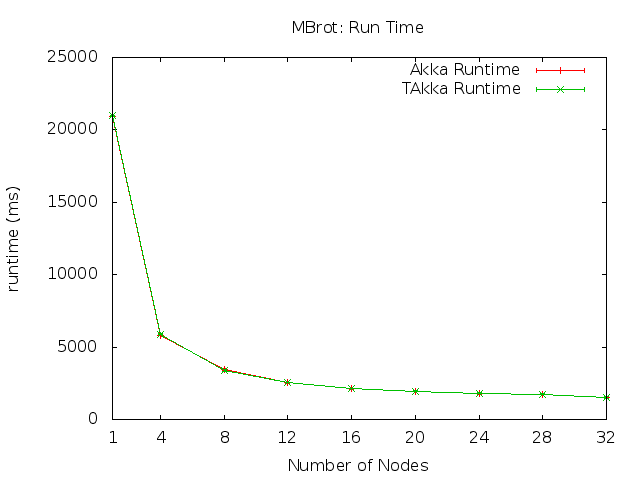
\includegraphics[scale=0.33]{MBrot_time.png}
        }
        \subfigure[]{
           \label{fig:second}
           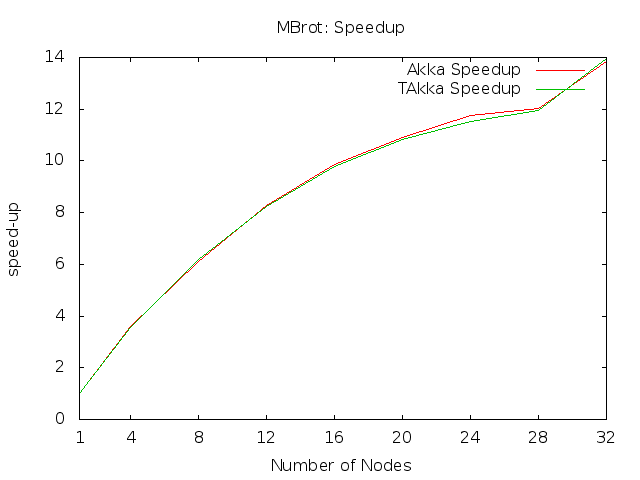
\includegraphics[scale=0.33]{MBrot_speedup.png}
        }\\
        \subfigure[]{
            \label{fig:third}
            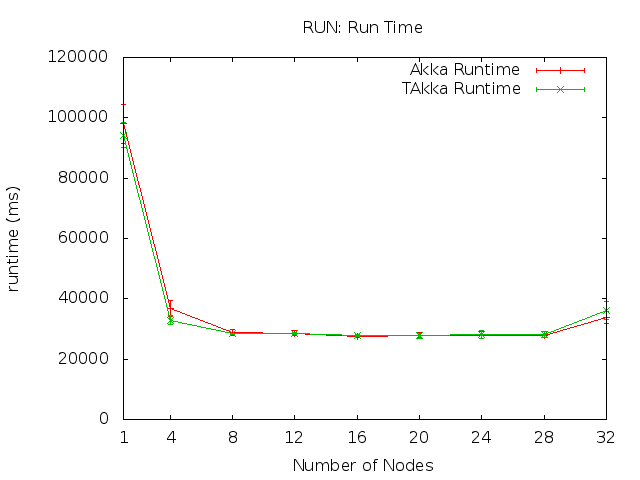
\includegraphics[scale=0.33]{RUN_time.png}
        }
        \subfigure[]{
            \label{fig:fourth}
            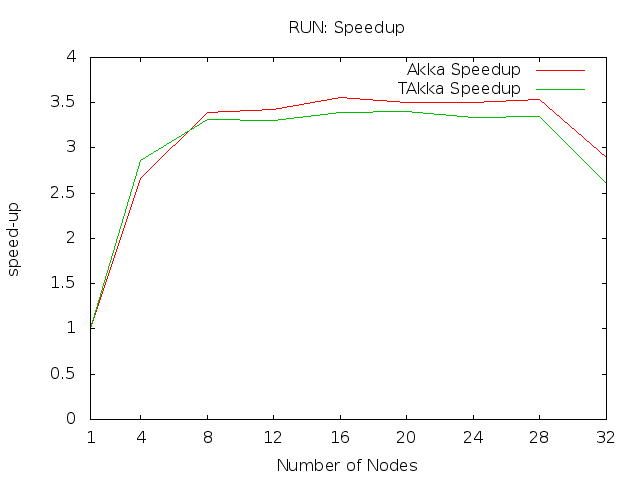
\includegraphics[scale=0.33]{RUN_speedup.png}
        }\\
        \subfigure[]{%
            \label{fig:fifth}
            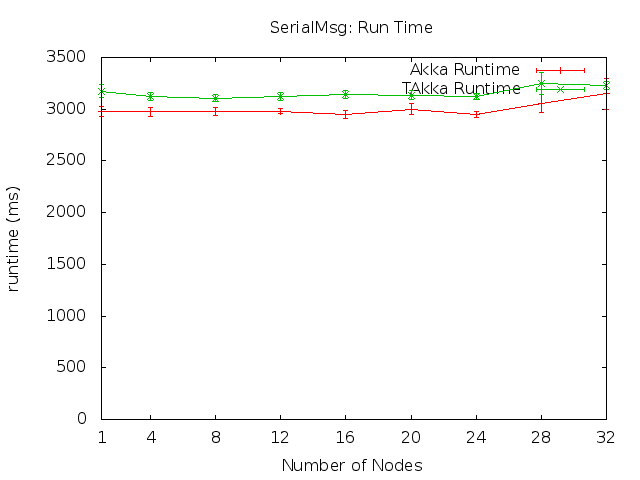
\includegraphics[scale=0.33]{SerialMsg_time.png}
        }
        \subfigure[]{%
            \label{fig:sixth}
            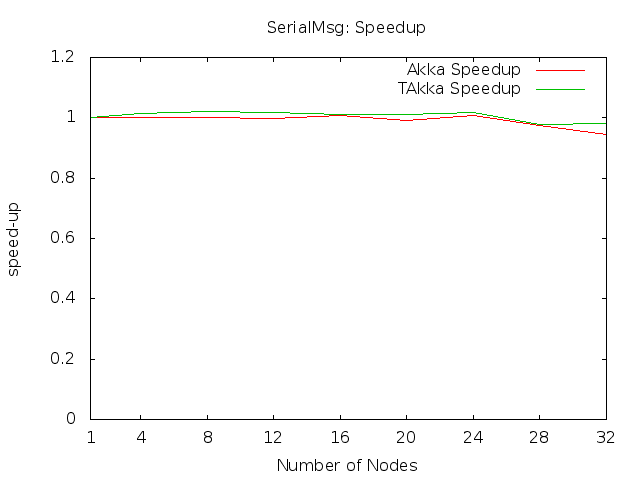
\includegraphics[scale=0.33]{SerialMsg_speedup.png}
        }\\
    \end{center}
    \caption{Efficiency and Scalability Benchmark}
   \label{scalability}
\end{figure}

\title{Assessing the Reliability \\of\\ Applications with Supervision Tree}
\author{ Jiansen HE }

% \date{\today}
\date{}
\documentclass[12pt, authoryear]{article}

\usepackage{comment}
\usepackage{natbib} 
%% \usepackage[style=alphabetic]{biblatex}
%% \usepackage[authoryear]{natbib}
%% \PassOptionsToPackage{authoryear}{natbib}
%% \usepackage{caption}
\usepackage{graphicx}
\usepackage{subfigure}
\usepackage{subcaption}
\usepackage{url}

\usepackage{paralist}
\usepackage[pdfpagelabels]{hyperref}
\usepackage[all]{hypcap}
\usepackage{verbatim}
\usepackage{array}
\usepackage{float}
\usepackage{multirow}
% \usepackage{rotating}
\usepackage{multicol}
\usepackage{longtable}


\begin{document}
\maketitle

\section{Introduction}\label{introduction}

Libraries such as Erlang OTP \citep{OTP}, Akka\citep{akka_doc}, and TAkka are 
built with the belief that the reliability of a software application can be 
improved by using supervision 
tree, in which failed components will be restarted by their supervisor.  Erlang 
OTP and Akka have been used in a number of applications that have achieved a
high reliability.  Could the reliability of a newly developed 
application be assessed in an effective manner? To what extend the usage of 
supervision tree contributes to the overall reliability?  

To answer above questions, this proposal suggests a research roadmap as follows.
Section \ref{methodology} summarizes general methodologies used in the area 
of reliability studies.  Focusing on the statistic approach to measure the 
reliability of software applications which are expected to have low failure 
rates, we propose to improve \citep{Littlewood93}'s single-run experiment, 
summarized in Section \ref{littlewood}, by using the iterative experiment 
(Section \ref{iterative}) when conditions apply.  The iterative approach can 
reduce the experiment time and can be stopped when the desired belief about the 
reliability had been rejected.  Aside from the methodology for directly 
assessing the reliability of a general application, this proposal also looks 
into approaches that indirectly assessing the reliability of application built 
using the supervision tree principle.   Section \ref{supervision} summarizes 
\citeauthor{JanHenry}'s approach for analysing the statical structure of Erlang 
supervision trees, and Jiansen's extensible work on dynamically monitoring 
TAkka supervision trees.  Finally, the essence of a node in a supervision tree 
is abstracted as a Deterministic Finite Automaton (DFA) in Section \ref{model}. 
The abstraction is used to model and compare designs of supervision tree in 
Erlang and (T)Akka, among alternatives that have not been adopted.  A 
straightforward definition for the reliabilities of a node in a supervision 
tree is derived from the model.  It remains to be seen whether i) the overall 
reliability of a supervising tree can be derived from the reliability of its 
nodes and the structure of that supervision tree, and ii) there exists an 
algorithm to aid the design of supervision tree with a high reliability.




\section{Methodologies for Assessing Software Reliability}\label{methodology}


The reliability in this proposal is defined as the probability that a system can
function properly for a specified period.  Formally, the reliability function, 
$R(t)$, denotes the probability that a system can function properly for time 
$t$.  In the study of software reliability, the period may be specified in term 
of {\it time units} (e.g. second) or {\it natural units} (e.g. number of 
operations) \citep{MusaBook}.  Reliability is usually reported in terms of  
failure rate ($\lambda$), Mean Time Between Failures (MTBF, $1/\lambda$), and 
other variants.  

The reliability function, its failure density function $f(t)$, and MTBF has 
following relationships: \citep{MusaBook}

$R(t) = \int_{0}^{\infty}f(x) dx$

$MTBF = \int_{0}^{\infty} tf(t)dt$

$MTBF = \int_{0}^{\infty} R(t)dt$


In literature, the precise definition of failures varies in the study of 
different systems.  Failure in this proposal is a general term to describe the 
situation where a system or a sub-system does not work as specified.

Once the meaning of failure is defined for a specific application, measuring 
the reliability during a period is straightforward.  The challenge 
is how to use the previous data, collected from experimental or operational 
environment, to give confidence about the reliability in the future under the
operational environment.

For software which involves iterative debugging process, software reliability 
growth models are usually employed to capture the relationship between the bug 
removing process and the reliability improvement.  \citep{Abdel-GhalyCL86} 
examines 10 models in this area, and a framework to evaluate the effectiveness 
of different models.

For software that has reached certain level of reliability and hence 
the debugging process has minor effects, \citep{Littlewood93} gives a 
Bayesian approach to validating its reliability.  Because this approach 
targets at systems that have high reliabilities, we will discuss this approach 
in sufficient detail in the next section.




\section{Statistic Approaches for Measuring Reliability}\label{statistic}

\subsection{Littlewood's approach to predict software 
reliability.}\label{littlewood}

The analysis in \citep{Littlewood93} answers the following question: given 
that $x$ failures are observed during the period of testing $t_0$,  what can we 
conclude about the reliability in the next $t$ time.
  
The two assumptions in Littlewood's approach are:

\begin{enumerate}[{Assumption} I)]
  \item the occurrence of failures is a poisson process, that is, time 
between failures are independent.
  \item the prior belief about the distribution of failure rate, $p(\lambda)$, 
follows the gamma distribution, Gam($\alpha, \beta$), where $\alpha$ and 
$\beta$ are positive hype-parameter that describes the sharp and the rate of 
the distribution.
\end{enumerate}

Assumption I is an appropriate choice for general studies.

Since the posterior belief is adjusted by the observed data, the prior belief 
will have less effect on the posterior belief if sufficient evidence is 
collected from a long experiment.  The Gamma distribution is chosen because it 
is the $conjugate\ distribution$ for poisson distribution.  It means 
that using the Gamma distribution as prior belief will result to a posterior 
belief which also follows the Gamma distribution.  Particularly, if the prior 
belief is Gam($a, b$), then posterior belief will be Gam($a+x, b+t_0$), where 
$x$ is the number of observed failures and $t_0$ is the experiment time. 
\citeauthor{Littlewood93}   Alternatively, any probability distribution may be 
used to replace the Gamma distribution, if it better describes the property of 
the failure rate of a particular application.  



\citeauthor{Littlewood93} then derives that the reliability function for the 
future $t$ time is

$ R(t | x, t_0) = \left ( \frac{b+t_0}{b+t_0+t} \right ) ^{a+x} $


\citeauthor{Littlewood93} then concludes that ``observing a long period of 
failure-free working does not in itself allow us to conclude that a system in 
ultra-reliable'' from the analysis of two extreme cases. 
The first case is, choosing an improper prior so that the posterior completely 
depends on the data.  The posterior itself is an proper distribution; however, 
after observing a period of failure-free operations, one has 50\% possibility 
to be failure-free for the same amount of time in the future.  The second 
example is, to claim a system has $10^6$ hours (114 years) MTBF by showing 
$10^3$ hours (41.7 days) of failure-free working, one must hold the prior 
belief that the system is a $10^6$ system.


\subsection {Reduce experiment time of the Littlewood and Strigini 
 test?}\label{iterative}

In \citeauthor{Littlewood93}'s study, prediction of the reliability is made 
according to the result of an earlier experiment under the same 
operational environment.  In such an experiment, even a long-time failure free 
observation cannot conclude a high reliability for the future. This section 
attempts to solve three problems: i) based on the same assumptions about the 
failure rate, can we improve the experiment so that the expected reliability 
can be verified or rejected earlier? ii) can we validate 
the same basic assumptions used in \citeauthor{Littlewood93}'s and the improved 
approach?  iii) is it possible to claim a genuine prior belief about the 
distribution of the failure rate?


\subsubsection{Iterative experiments}

Assuming that the occurrence of failures is a poission process and the failure 
rate follows the Gamma distribution, representing the Gamma distribution using 
hyper-parameters, it is clear that the posterior belief about the failure rate, 
$Gam(a+x, b+t)$, depends on the prior belief $Gam(a,b)$, the 
$total$ number of observed failures $x$, and the $total$ 
experiment time $t$.  Therefore, for an application that consists of a number 
of replica subsystems, we can replace \citeauthor{Littlewood93}'s experiment 
with an equivalent iterative experiment described below.

An iterative experiment consists of several rounds of sub-experiments, each of 
which may consists of several parallel experiments.  In an iterative 
experiment, the posterior belief of one round is used as the 
prior belief of the next round.  Instead of asking whether a system will be 
reliable in the next $10^6$ hours based on the failure rate of the first $10^3$ 
hours \citep{Littlewood93}, the experiment conductor concerns whether the 
system will be reliable in 
the next round, based on the failure rate of previous results.  In 
each iteration, a number of instances may be tested in parallel to collect the 
results of more instance hours within less time.  An iterative experiment may 
be stopped as soon as the belief about the failure rate is disproved, or the 
base assumption about poisson process and Gamma distribution are rejected.

Take the above proposal into practise, assuming we are asked to test whether 
a distributed web service designed for an organisation will be as reliable as 
its developers claimed for the next a few years.  We may run a test on one or 
two local machines for 1 day.  If the result meets the requirement, then we may 
test the application on some servers of the organisation for half a week.  
Then, we may rent 1000 similar servers from one or more cloud service providers 
in the third round which lasts a week.  By doing this, we can collect the 
number of failures occurred in an experiment of 168,000 instance hours within 
a week ($168,000 = 7 \times 24 \times 100$) .  Fortunately, the data can be 
treated as equivalent to a result 
collected from a single-run experiment on one machine for 19 years ($19 = 
168,000 \div 24 \div 365$) , if our assumptions are valid for tested system.  
Renting a thousand server instances might be expensive, but the risk of wasting 
resource on testing application that doesn't meet the desired reliability has 
been reduced in previous rounds of tests.


\subsubsection{Verify Assumptions}

Both \citeauthor{Littlewood93}'s original approach and our alternative are based 
on the assumption that the occurrence of failures is a poisson process and the 
failure rate follows a Gamma distribution represented by two 
hyper-parameters.  Those two assumings are good choice in a study for general 
purposes.  For a test of a real application, to what extend can we rely on the 
assumption of poisson process and the prior belief with guessed 
hyper-parameters?  To verify those assumptions, suitable goodness-of-fit tests 
can be used.  Following are example approaches.


To verify the assumption on poission process, we can alternatively check 
whether the number of failures in consecutive fixed periods follows the 
poission distribution, whose mean and variance are the same.  To verify the 
assumption on gamma distribution, \citep{GammaFIT} gives improved methodologies 
for the purpose of reliability test.


\subsubsection{Obtain a genuine prior belief}

Following is my guesswork. Appropriate statistic analysis is required.

If $x$ failures are observed in the previous experiment of $t$ time and the 
base assumption cannot be rejected by the data in previous tests, the 
{\bf best} prior belief for the next iteration is assuming the distribution of 
failure rate $\lambda$ follows Gam($x$, $t$).

This is a significant difference between the iterative experiment and 
\citeauthor{Littlewood93}'s single run experiment.  In 
\citeauthor{Littlewood93}'s approach, claiming a Gam($x$, $t$) {\it posterior} 
is the same as claiming a improper $prior$ Gam($a$, $b$), where $a,\ b\ 
\rightarrow 0$.  In an iterative experiment, the first round can be used to 
``generate'' a reliable prior for the second round.  However, at least 1 failure 
need to be observed in the first round because $a$ and $b$ in Gamma distribution 
are positive numbers.  In a ultra-reliable system, waiting for the first 
occurrence of failure may take a long time.


\subsubsection{Testing in adversely environment.}

Another attempt to give a reliability prediction in short period is testing 
the system in adversely environment.  This idea, known as accelerated testing 
(AT), has been explored in hardware reliability test for years 
\citep{Escobar06areview}, and has been applied to test the $FASTAR^{SM}$ 
platform, a set of systems used to automatically  restore the AT\&T 
network\citep{CukicSoft}.

An accelerated test consists of two general steps.  The first step is to 
identify accelerating factors (e.g. temperature, workload, temperature etc.) and 
run the experiment.  The second step is to use suitable regression model to 
predict the reliability in normal condition.  

The significance of an accelerated testing depends on the choice of the 
regression model.  For a hardware, the relationship between its life-time 
and environment factors (e.g. temperature) has been well studied.  In the 
$FASTAR^{SM}$ test, to capture and verify the regression model, 32 runs are 
carried out under different pressure environment.  Each run lasts for about 30 
hours and a few failures are observed during the test.  

Bring in the same idea into the test of TAkka applications, for example, with 
the help of the Chaos Monkey library, can we effectively test the reliability 
within a reasonable short period?  Unfortunately not.  

Let's run two experiments in parallel.  In one experiment, ChaosMonkey is not 
used and its failure rate, $\lambda_n$, is assumed to be the same as in the 
normal operational environment. In the other experiment, ChaosMonkey is 
employed to increase the exception rate so that the failure rate, $\lambda_c$, 
will be higher than $\lambda_n$.  Failure rates in the two experiments are 
linked by the following equation:
$\lambda_n \times t_n = \lambda_c \times t_c$, where $t_n$ and $t_c$ are expect 
periods of seeing $x$ failures in the normal environment and in the ChaosMonkey 
test.

The above equation shows that the expected time for the $nth$ occurrence of 
failures decreases when its failure rate increased.  Therefore, assumptions 
on the poission process and the Gamma distribution can be verified in shorter 
time.  From a serials of ChaosMonkey test with different failure rates, we may 
fortunately find that the occurrence of failures in the tested application is 
always a poission process.  As a result, to measure its reliability in normal 
operational environment, only a small number of errors need to be observed 
under the test in normal environment.  However, it may take a long time to 
observe the first occurrence of failures in a system whose MTBF is $10^6$ 
hours.




\section{Reliability Studies on Supervision Tree}\label{supervision}

\subsection{Static Analysis on Tree Structure}\label{Static}

Based on the Core Erlang Language defined by \citep{CoreErlang}, 
\citep{JanHenry} defines an abstract semantic to extract structures of Erlang 
programs.  Since supervision tree is constructed in Erlang by calling callback 
functions in the {\it supervision} module, \citeauthor{JanHenry}'s work can 
be used to abstract the structure of supervision trees form the source code of 
Erlang applications.

Noted in the later part of \citeauthor{JanHenry}'s thesis, there are two 
limitations of his approach.  Firstly, the abstraction only captures the static 
structure of the supervision tree, which may differ from its run-time 
structure.  Secondly this approach requires specialised knowledge about the 
Erlang language and only applies to ``applications that have been 
designed according to the suggestion of the OTP documentation and using the OTP 
library behavious.'' \citep{JanHenry}.



\subsection{Dynamic Monitoring}\label{Dynamic}

The supervision view library in the TAkka paper.




\section{Modelling Supervision Tree}\label{model}


To study properties of supervision tree, a simple formal model is required to 
describe the essence of supervision tree.  Section \ref{DFA}
models Worker and Supervisor and Deterministic Finite Automata (DFA).  With 
this model, implementation alternatives of Supervision Tree are compared.  More 
importantly, the model helps us to give a simple general definition for the 
reliability of nodes in a supervision tree.  This section ends with a proposal 
for investigating the reliability of a supervision tree, based on the 
reliabilities of its nodes and the relationships between nodes.


\begin{comment}
The model shall not include 

The model shall contain the minimum 
number of constructs and small-step semantics that describes supervision.  
Operations related to supervision are separated from functions and 
message-passing for general purpose.  The simple model will be used to compared 
core Erlang (where supervision is optional), Akka (where supervision is 
obligatory), and TAkka (where messages are typed).  Since Akka and TAkka don't 
have a formal model, giving a model that can be used to describe/check their 
properties is a non-trivial contribution.


In addition, a stack of failure models will be defined.  We will examine 
failures that are typically handled at hardware level, OS level, VM level, and 
the application level.  Presumably, supervision injects a layer between the 
application and the VM, and automates the recovery of some failures previously 
handled by programmers at the application level (e.g. exception).
\end{comment}

\subsection{Worker and Supervisor as Deterministic Finite Automata (DFA)} 
\label{DFA}

Figure \ref{fig:DFA} gives state graphs of DFAs that describe 
worker and supervisor in a supervision tree.  Nodes in the graphs represent 
states of that DFA and arrows are transitions from one state to another.  A 
transition is triggered either by the node itself or due to changes of the 
environment it resides.

At any time, a worker may be in one of its four states: {\bf Start}, {\bf 
Free}, {\bf Blocked}, or {\bf Dead}.  After automatically being initialised to 
the {\bf Free} state, the Work can accept messages from its outside 
environment and enters to the {\bf Blocked} state where no messages will be 
processed.  If no error occurred when processing the message, the worker emits 
a result and go back to the {\bf Free} state.  An error may occur during the 
middle of message processing (e.g. software bugs) or when the environment 
changes (e.g. hardware failures), in which cases the worker reports its failure 
to its supervisor and go to the {\bf Dead} state.  A dead worker can be resumed 
or restarted by its supervisor so that it can process new messages.  {\bf Free} 
and {\bf Dead} are marked as accept states from which no further actions may 
occur.  On the contrary, a {\bf Blocked} worker will eventually emit a reply 
message or raise an exception; and all workers will be successfully initialised.

The DFA of a supervisor whose only duty is supervising its children is given in
Figure \ref{fig:2}.  A supervisor in its {\bf Free} state reacts to failure 
messages from its children.  Meanwhile, a supervisor may fail at any time 
and reports its failure to its supervisor.

\begin{figure}[p]
     \centering 
        \subfigure[Worker]{
            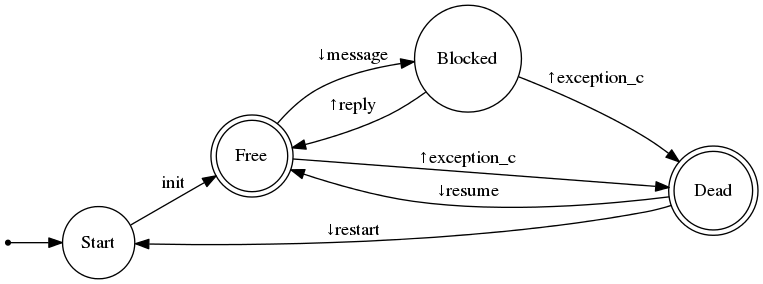
\includegraphics[scale=0.5]{child.png}
%            \caption{A gull}
            \label{fig:1}
        }\\
        \subfigure[Supervisor]{
           \label{fig:2}
           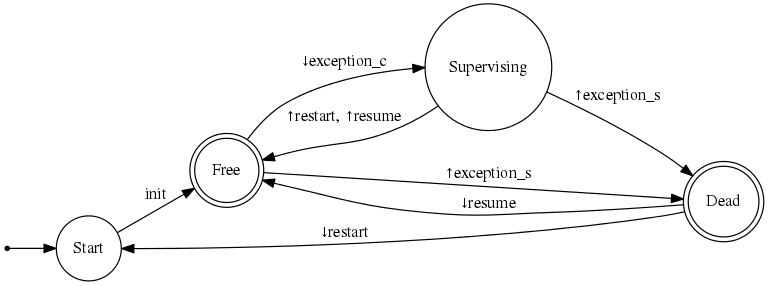
\includegraphics[scale=0.5]{supervisor.png}
        }\\
  \caption{Worker and Supervisor as Deterministic Finite Automata}
  \label{fig:DFA}        
\end{figure}

\subsection{Implementation Considerations}

The two DFAs given in Figure \ref{fig:DFA} are abstracted for theoretical 
study.  In an implementation of the supervision tree model, following issues 
might be considered.

\paragraph{Distributed Deployment}
Supervision Tree represents the logic relationship between nodes.  In 
practice, nodes of a supervision tree may be deployed in distributed machines.  
A child node may be restarted at or shipped to another physical or virtual 
machine but stays in the same place in the logic supervision tree.


\paragraph{Heart-Beat Message}  At run-time, failures may occur at any time for 
different reasons.  In some circumstances, failure messages of a child may not 
be delivered to its supervisor, or even worse, not sent by the failed child at 
all.  To built a system tolerant to the above failures, supervisors need to be 
aware of the liveness of their children.  One approach to achieve this is 
asking the child periodically sending heart-beat message to its supervisor.  
If no heart-beat message is received from a child for some consecutive 
periods, that child is considered dead by the supervisor and an appropriate 
recovery process is activated.  In the model, a 
logical exception is sent from a child to its supervisor when no heart-beat 
message is delivered within a time-out, and a restart or resume message is sent 
to a suitable machine where the node will reside.


\paragraph{Message Queuing}
In the simplified model given in Figure \ref{fig:1}, a worker can processed one 
message a time when it is {\bf Free}.  The model does not exclude the case 
where messages are queuing either in memory or a distributed database.  
Similarly, when a worker is resumed from the failure of processing a message, 
the message it was processing may be retrieved from a cache or be discarded.




\subsection{Unifying Supervisor and Worker}

Notice that the model for supervisor and worker are similar if exceptions from 
the child is viewed as request messages to a supervisor and restart/resume 
is viewed as reply messages to a child.  Can we defined a $combined$ node which 
can be both a worker for a task and a supervisor for some children? Of course 
we can, as what have been implemented in Akka\citep{akka_doc} and inherited by 
TAkka. The rest of this sub-section will compare three strategies of unifying 
supervisor and worker.

\paragraph{Supervisor as a Worker}  In the design of Akka, messages to 
actors are not typed.  An Akka actor therefore can be both a supervisor and a 
worker.  To model an Akka actor, only Figure \ref{fig:1} is required.

\paragraph{Combining Supervisor and Worker}  The TAkka library inherits the 
implementation of Akka, but separates messages for supervision purpose from 
messages for general purposes so that an actor can be parameterized by the 
type of message it expects.  A more precise model for a TAkka actor is given in 
Figure \ref{fig:3}.  Both Akka actor and TAkka actor can only be a supervisor 
or a worker at a time.  As a result, the supervision task may be blocked until 
the end of another computational task.


\paragraph{Supervisor in Parallel with Worker}  One way to get around the 
limitation of Akka and TAkka's design is place the supervision process and the 
worker process in parallel, as shown in Figure \ref{fig:4}.  From the 
perspective of model analysis, the above parallel model is equivalent to the 
one which separates the supervisor process and the worker process into two 
nodes, and treat them as siblings or a supervisor and a child.



\begin{figure}
%  \ContinuedFloat 
  \centering         
        \subfigure[Supervisor AND Worker]{
            \label{fig:3}
            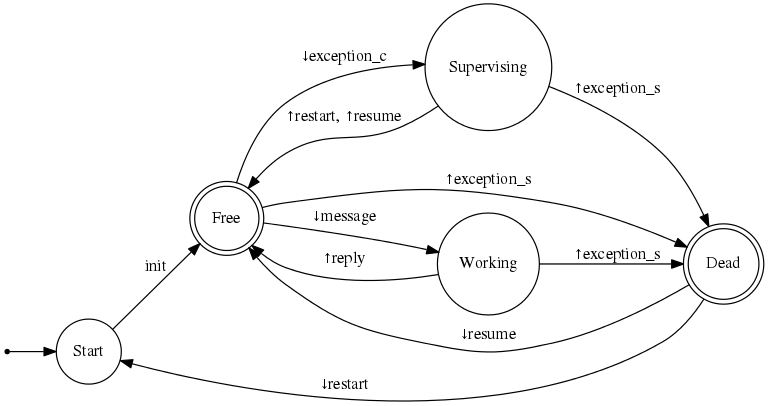
\includegraphics[scale=0.5]{supervisorANDchild.png}
        }\\
        \subfigure[Supervisor PAR Worker]{
            \label{fig:4}
            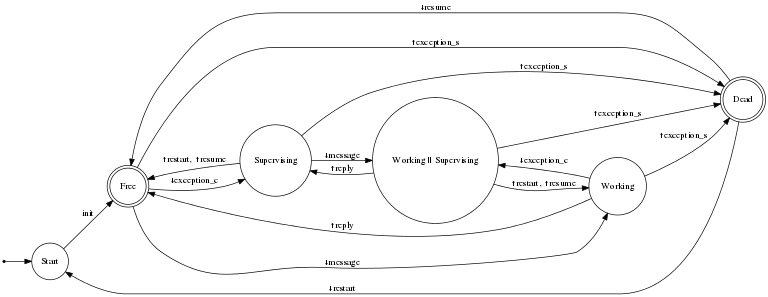
\includegraphics[scale=0.5]{supervisorPARchild.png}
        }\\
    \caption{A Node that Unifies Supervisor and Worker}
   \label{fig:unify}
\end{figure}


To summarize, a node that naively combining the role of supervisor and worker 
(Figure \ref{fig:1} and \ref{fig:3}) has less availability than a node that 
place the supervision process and the worker process in parallel processes 
(Figure \ref{fig:4}).  Interestingly, during the process of designing TAkka, we 
realized that the type of supervision messages should be separated 
from the type of other messages.  However, partly because we would like to 
reuse the Akka implementation and partly because we did not have the above 
model at that time, the process of handling supervision messages is not 
separated from the process of handling other messages.


\subsection{Reliability of a Node}

The reliability of a node, either a worker or a supervisor, is defined as:

The the probability that a node is in the {\bf Free} state.


\subsection{Reliability of a Supervision Tree}

A supervision tree in this proposal consists of workers and supervisors defined 
in Figure \ref{fig:1} and Figure \ref{fig:2} respectively.  A node that 
combines a supervisor and a worker is separated into two nodes, together with a 
constraint that one node will fail when the other fails.

The reliability of a supervision tree may be derived from following factors:

\begin{itemize}
  \item The reliabilities of all workers.  Although testing the reliability of 
a system with low failure rate is difficult or even impractical, the 
reliability of an individual component may be measured within a reasonable 
short time. 
  \item The reliability of a supervisor.  The reliability of a supervisor 
process may be tested as part of the library development process.
  \item The relationship between nodes.  Nodes in a supervision tree may 
collaborate to perform a task or to achieve a higher reliability. The 
reliability of a supervising shall capture complex relationships 
between nodes.
\end{itemize}

The experiment proposed in section \ref{iterative} may to used to measure the 
reliabilities of individual nodes in a supervision tree.  To obtain the 
reliability of a supervision tree, when direct measurement becomes impractical, 
knowledge about constraints between nodes are required.  

I propose to investigate following problems in the next stage:

\begin{itemize}
  \item What are possible constraints between nodes?  For each constraint, what 
is the algebraic relationship between the reliability of a sub-tree and 
reliabilities of individual nodes?
  \item Based on the above result, how to calculate the overall reliabilities 
of a supervision tree?  When is the reliability is improved by using 
supervising tree, and when not?
  \item Given the reliabilities of individual workers and constraints between 
them, is there an algorithm to give a supervision tree that improves the 
reliability?  If not, can we determine if the desired reliability is not 
achievable? 
\end{itemize}


\bibliographystyle{abbrvnat}
\bibliography{reliability}

\end{document}


\section{Conclusion}

Existing actor libraries accept dynamically typed messages.  The TAkka
library introduces a type-parameter for actor-related classes. The additional 
type-parameter of a TAkka actor specifies the communication interface of 
that actor.  With the help of type-parameterized actors, unexpected 
messages to actors are rejected at compile time.

In addition to eliminating programming bugs and type errors, 
programmers would like to have a failure recovery mechanism for
unexpected run-time errors.  We are glad to see that type-parameterized 
actors can form supervision trees in the same way as untyped actors.

Lastly, test results show that building type-parameterized actors on top of 
Akka does not introduce significant overheads, with respect to program size,
efficiency, and scalability.  In addition, debugging techniques such 
as Chaos Monkey and Supervision View can be applied to applications built 
using actors with supervision trees.  The above results encourage the use of 
types and supervision trees to implement reliable applications and improve the 
reliability of legacy applications with little effort.  We expect similar 
results can be obtained in other actor libraries such as future extensions 
of CloudHaskell \cite{OTPCloudHaskell}.

\acks
Acknowledgments


\bibliographystyle{abbrvnat}
\bibliography{takka}

\appendix
%  \section{Examples for Expressiveness and Correctness Test}
\label{app_correct}

\begin{description}
  \item[ATM simulator\cite{quviq} ] A bank ATM simulator with backend database
and frontend GUI.
  \item[Elevator Controller \cite{quviq}] A system that monitors and schedules a
number of elevators. 
  \item[Ping Pong \cite{akka_doc} ] A simple message passing application.
  \item[Dining Philosophers \cite{akka_doc}] A application that simulates the
dining philosophers problem using Finite State Machine (FSM) model.
  \item[Distributed Calculator \cite{akka_doc}] An application that examines
distributed computation and hot code swap.
  \item[Fault Tolerance \cite{akka_doc}] An application that demonstrates how
system responses to component failures.
  \item[Barber Shop\cite{BarberShop} ] A application that simulates the Barber
Shop problem. 
  \item[EnMAS \cite{EnMAS}] An environment and simulation framework for
multi-agent and team-based artificial intelligence research

  \item[Socko Web Server \cite{SOCKO} ]  lightweight Scala web server that can
serve static files and support RESTful APIs
  \item[Gatling \cite{Gatling}] A stress testing tool.
\end{description}


\section{Examples for Efficiency and Scalability Test}

\begin{description}
  \item [bang] This benchmark tests many-to-one message passing.  The benchmark
spawns a specified number sender and one receiver.  Each sender sends a
specified number of messages to the receiver.
  \item [big] This benchmark tests many-to-many message passing.  The benchmark
creates a number of actors that exchange ping and pong messages.
  \item [ehb] This is a benchmark and stress test.  The benchmark is
parameterized by the number of groups and the number of messages sent from each
sender to each receiver in the same group.
  \item [mbrot] This benchmark models pixels in a 2-D image.  For each pixel,
the benchmark calculates whether the point belongs to the Mandelbrot set.
  \item [parallel] This benchmark spawns a number of processes, where a list of
N timestamps is concurrently created.
  \item [genstress] This benchmark is similar to the bang test.  It spawns an
echo server and a number of clients.  Each client sends some dummy messages to
the server and waits for its response.  The Erlang version of this test can be
executed with or without using the gen\_server behaviour.  For generality, this
benchmark only tests the version without using gen\_server.
  \item [serialmsg] This benchmark tests message forwarding through a
dispatcher.
  \item [timer\_wheel] This benchmark is a modification to the big test.  While
responding to ping messages, a process in this message also waits pong messages.
 If no pong message is received within the specified timeout, the process
terminates itself.
  \item [ran] This benchmark spawns a number of processes.  Each process
generates a list of ten thousand random integers, sorts the list and sends the
first half of the result list to the parent process.
\end{description}

% \received{September 2008}{March 2009}

\end{document}


